\documentclass{scrartcl}
\usepackage{graphicx}
\usepackage{subcaption}
\usepackage{graphics}

\usepackage{listings}
\usepackage{color}

\renewcommand\lstlistingname{Quelltext} % Change language of section name

\lstset{ % General setup for the package
language=Python,
basicstyle=\small\sffamily,
numbers=left,
numberstyle=\tiny,
frame=tb,
tabsize=4,
columns=fixed,
showstringspaces=false,
showtabs=false,
keepspaces,
commentstyle=\color{red},
keywordstyle=\color{blue}
}

\makeatletter
\renewcommand\subparagraph{%
\@startsection {subparagraph}{5}{\z@ }{3.25ex \@plus 1ex
\@minus .2ex}{-1em}{\normalfont \normalsize \bfseries }}%
\makeatother

\begin{document}

\title{Semantic Role Labelling}
\subtitle{Final project for Natural Language
Processing by Prof. Roberto Navigli}
\author{Son Tung Nguyen}

\maketitle

\section{Introduction}
Semantic Role Labelling (SRL), first proposed by \cite{ARTICLE:2}, is the task of identifying
the arguments for one specific predicate among all the words in the sentence. Answering the
question "who did what to whom?", solving SRL task was proved to be beneficial to many NLP
applications. Figure 1 shows an example of a SRL task, that is to find out the roles of
arguments "I" and "the computer" are "A0" and "A1" of the predicate "repair".
\begin{figure}[h!]
\centering
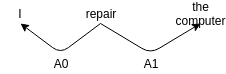
\includegraphics[width=200]{figures/fig1.png}
\caption{A semantic role labelling example.}
\label{fig:srl}
\end{figure}

\section{State of the art}
Long short term memory (LSTM) was showed to be very effective in tackling SRL problem. One of the first system
to use LSTM outperformed previous methods and was a huge success \cite{ARTICLE:1}. Since then, many improvements
have been made to increase the performance further. \cite{ARTICLE:3} exploited other information of the sentence (POS, dependency
relation) and found them to be beneficial when solving SRL. Another more recent system used Highway connection
and constrained A* decoding \cite{ARTICLE:4}.
\section{Proposed method}

\subsection{Model architecture}
Used model architecture was closely followed by \cite{ARTICLE:1}. The input to the model
was in shape of $[\ batch \ size, sequence \ length, 251 \ ].$ That means for each
word in a sentence, the following information was passed:
\begin{itemize}
\item Currently processed word (in form of a 50d vector).
\item Lemma of currently processed predicate (in form of a 50d vector).
\item Predicate context (in form of a 50d vector).
\item A binary number indicating that current word was in predicate context.
\item POS index indicating the POS tag of current word.
\item DEP index indicating the dependency of current word to predicate.
\end{itemize}

\noindent
All the above information were concatenated together to produce a single vector
of 251 entries.
Then, a LSTM of state size 64 was used to capture the sequential relationship of the sentence.
The output of this LSTM layer was then connected to a fully-connected layer
before forwarded to Conditional Random Fields (CRF) \cite{a7} layer to compute the loss.
This simple model alone could achieve a F1 score of 0.55 on the development set
without using any additional information from POS tagging or dependency (DEP).
\subsection{Improvements}

\subparagraph{Stack more LSTM layers}
The network was modified from LSTMCell to MultiRNNCell to support multi LSTM
layers. Table \ref{t1} shows that when using MultiRNNCell with 2 layer F1 score went up to
0.59 but decreased to 0.55 for 3 layers.
\subparagraph{Bigger predicate window}
Predicate window size was experimented to see if bigger size would lead to better
F1 score. The result was not as expected since bigger predicate window size did
not have a big positive effect on F1 score.
\subparagraph{POS and DEP information}
POS and DEP information were also integrated into the input vector to see if
there would be any improvement. There were 48 POS types and 69 DEP types. Each type
was encoded by a unique number from 0 to 47 (for POS) and 0 to 68 (for DEP). We can see
using POS information helped quite well (F1 score increased from 0.55 to 0.58). This can
be further enhanced with DEP information (0.59).
\subparagraph{Bi LSTM architecture}
I tried to apply Bi-LSTM architecture using \cite{a9}. The network architecture
was basically from the input layer to the first linear layer which was activated
be a tanh function. The output of this layer then was forwarded to LSTM layers to
be processed in both directions. After this, the concatenated h vectors went to
another tanh-linear layer and a linear layer. Finally, the CRF layer took over to
compute the loss and make inference. This new architecture did not work for me as
it only achieved a F1 score of 0.57.


\section{Experiments}
\subparagraph{Datasets}

Dataset using in experiments was CONLL 2009 \cite{a5}. This dataset was split
into train set and development set for training and testing the model.
\subparagraph{Word vectors}
Pretrained GLOVE vectors \cite{a6} was used. Each word corresponded to one vector of
size 50d. If there was not any match for a word, this word would get a fixed
random vector (UNK vector). About 0.6 percent of the words were unknown.
\subparagraph{Training settings}
A learning rate $lr_{1} = 0.1$ was used to train the model. The loss was optimized by
a Gradient Descent optimizer \cite{a8} for 5 epochs.

\section{Evaluation}
All models and methods were evaluated on the development set by F1 metrics. F1
score was calculated by two additional metrics: precision and recall. However,
in order to compute precision and recall, I first counted the number of true
positives (TP), false positives (FP) and false negatives (FN). The rule for counting
was basically summarized as the following code.
\begin{lstlisting}
if gold[h] == pred[h] and gold[h] != CLASSES["_"]:
    TP += 1
elif gold[h] != pred[h] and pred[h] != CLASSES["_"]:
    FP += 1
elif gold[h] != pred[h] and pred[h] == CLASSES["_"]:
    FN += 1
\end{lstlisting}
After we have TP, FP and FN, precision, recall and F1 score are computed as below:
\newline
\begin{align*}

$precision &= \frac{TP}{TP+FP}\\$

$recall &= \frac{TP}{TP+FN}\\$

$F1 &= 2\cdot\frac{precision \times recall }{precision+recall}$

$ $
\end{align*}
\newline
Based on this evaluation scheme, my best model had F1 score, precision and recall
of 0.63, 0.67 and 0.59, respectively. Recall was lower than precision score. This
meaned the model mislabelled more words as negatives (null label) resulting in a higher FN.
Figure 2 and Figure 3 represents confusion matrix on the ten most popular classes,
which give us a closer look on how the model performed.

\newpage
\begin{table}[h!]
\begin{center}
\caption{Summarisation of multiple methods.}
\label{t1}
\resizebox{\columnwidth}{!}{
\begin{tabular}{l|c|c|c|c|c|c|c|c}
\textbf{Model} & \textbf{Pred window size} & \textbf{Number of LSTM layers} & \textbf{Using POS} & \textbf{Using DEP} & \textbf{F1 score}\\
\hline
LSTMCell & 1 & 1 & No & No & 0.558\\
LSTMCell & 2 & 1 & No & No & 0.574\\
LSTMCell & 3 & 1 & No & No & 0.54\\

LSTMCell & 3 & 1 & Yes & No & 0.583\\
LSTMCell & 3 & 1 & No & Yes & 0.558\\
LSTMCell & 3 & 1 & Yes & Yes & 0.59\\

MultiRNNCell & 1 & 1 & No & No & 0.55\\
MultiRNNCell & 1 & 2 & No & No & 0.59\\
MultiRNNCell & 1 & 3 & No & No & 0.55\\
MultiRNNCell & 3 & 2 & Yes & Yes & 0.63\\

Bi-LSTM & 1 & 1 & No & No & 0.57

\end{tabular}
}
\end{center}
\end{table}

\begin{figure}[h!]
\centering
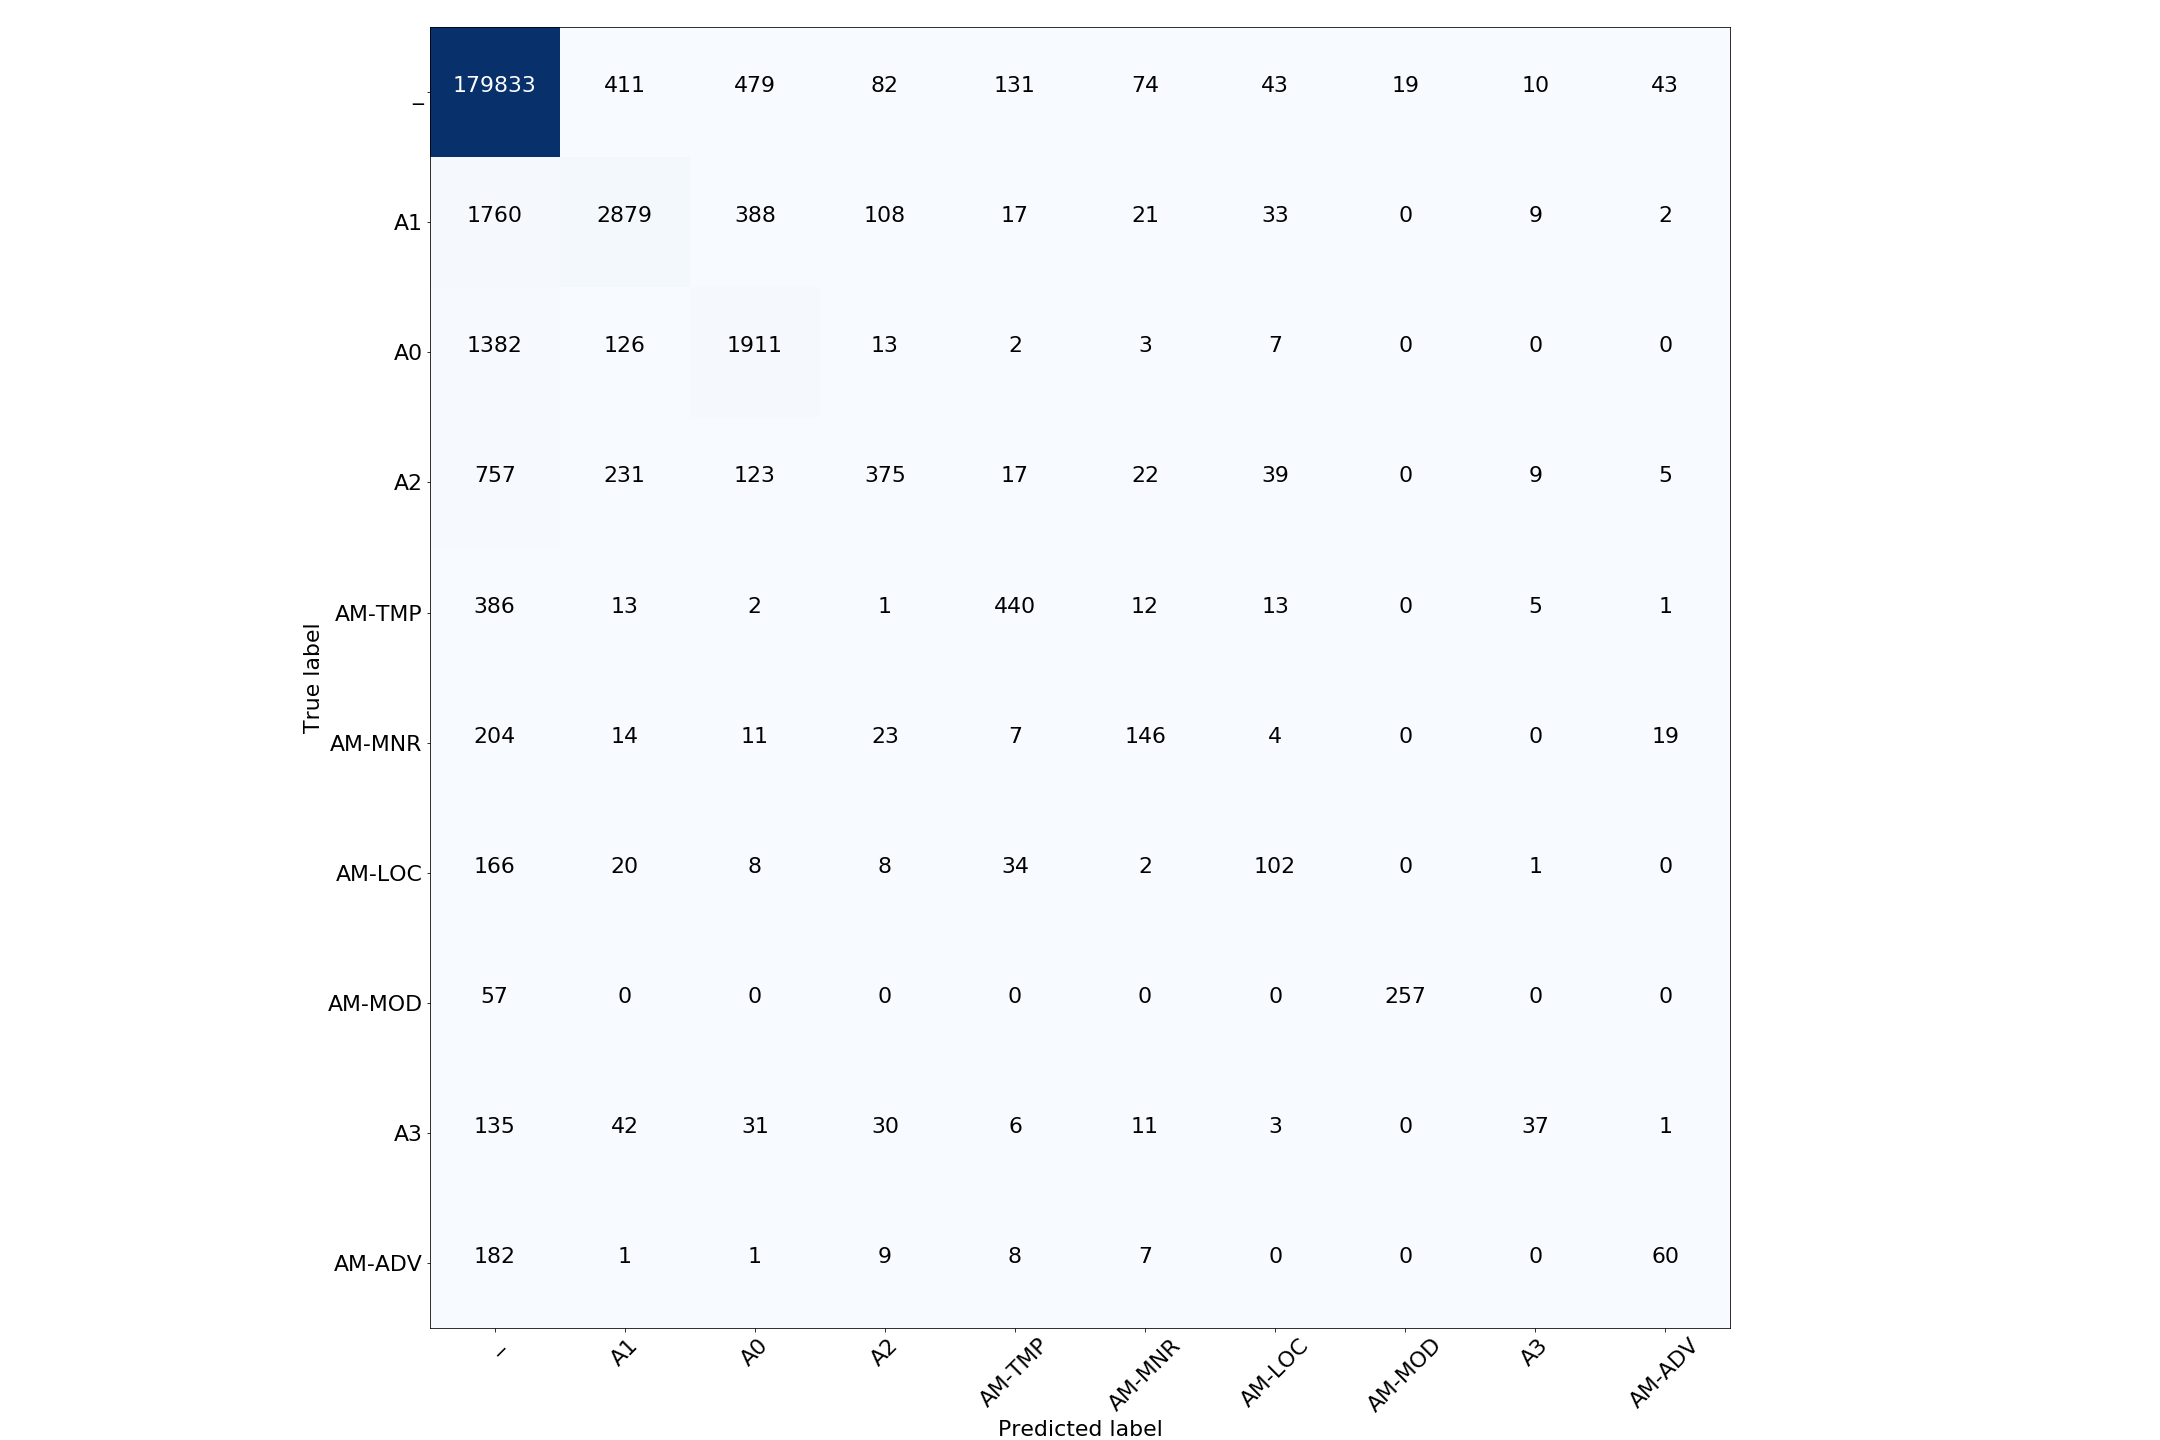
\includegraphics[width=400]{figures/fig2.png}
\caption{Confusion matrix of 10 most popular classes in the development set.}
\label{fig:2}
\end{figure}

\begin{figure}[h!]
\centering
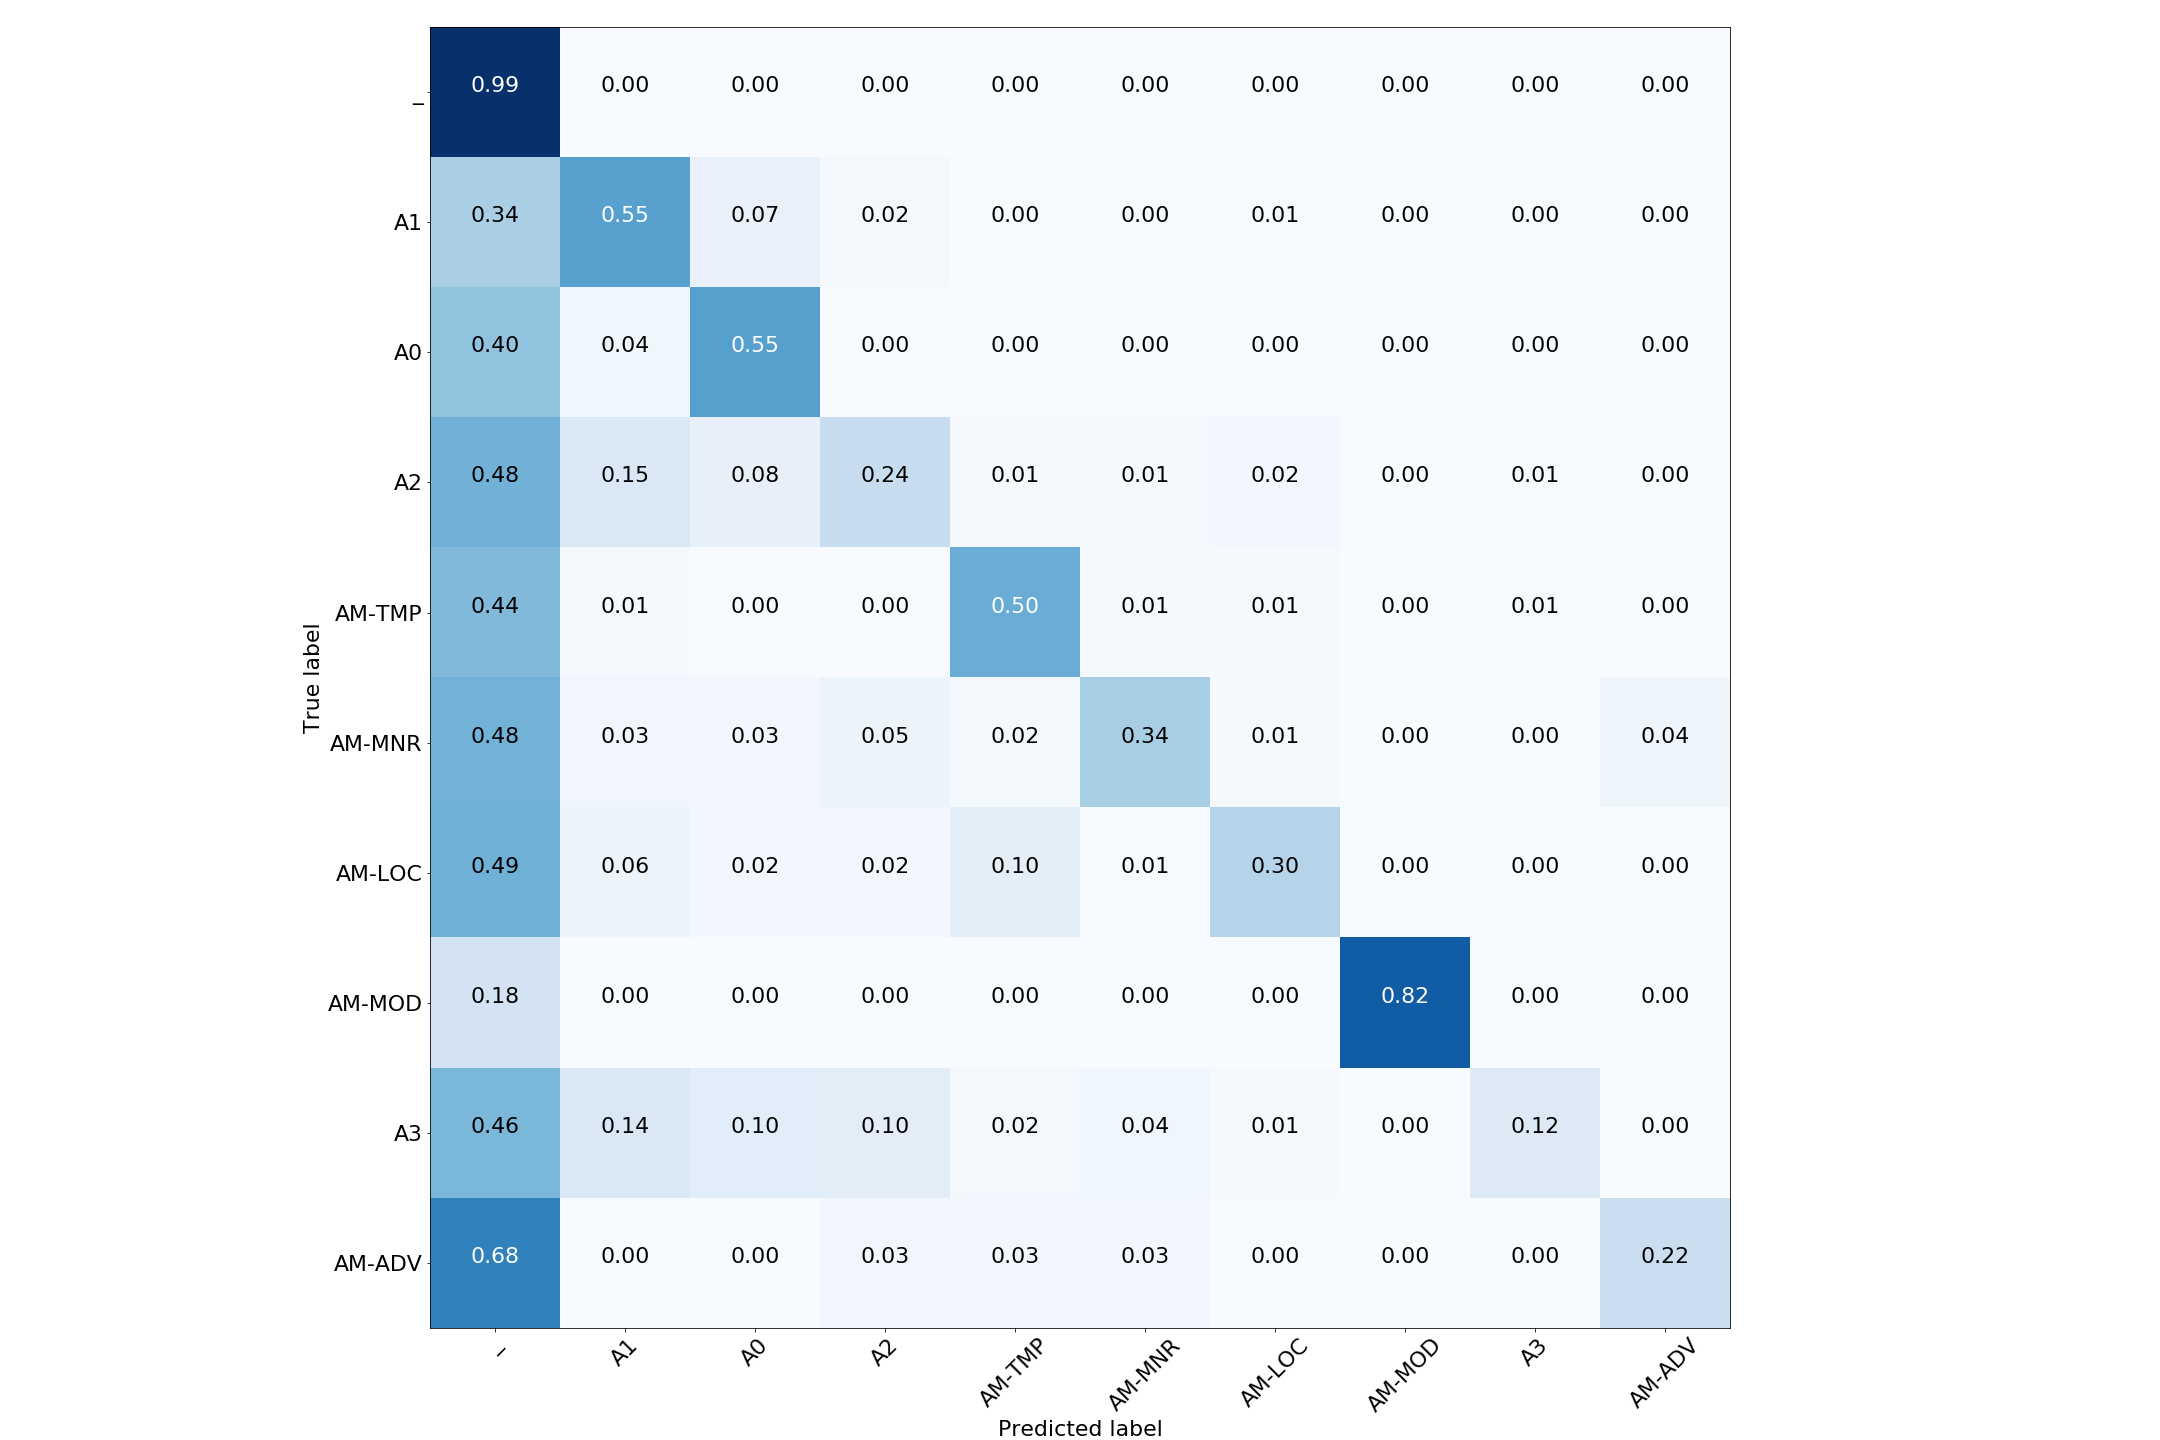
\includegraphics[width=400]{figures/fig3.png}
\caption{Normalized confusion matrix of 10 most popular classes in the development set.}
\label{fig:3}
\end{figure}

\clearpage
\bibliography{ref}
\bibliographystyle{ieeetr}

\end{document}
